%<<setup-child, include = FALSE>>=
%library(knitr)
%library(microbenchmark)
%library(snow)
%library(colorspace)
%library(ggplot2)
%library(zoo)
%library(gridExtra)
%source("rsrc/functions.R")

%# mutate = ecr::mutate

%set_parent("../style/preamble.Rnw")
%@

\input{../../style/preamble}
\input{../../latex-math/basic-math}
\input{../../latex-math/basic-ml}
\input{../../latex-math/ml-nn}


%\newcommand{\titlefigure}{figure_man/}
\newcommand{\learninggoals}{
\item LEARNING GOAL 1
\item LEARNING GOAL 2}


%\usepackage{animate} % only use if you want the animation for Taylor2D

\title{Optimization}
%\author{}
%\date{}

\begin{document}

\lecturechapter{First order methods: Gradient descent}
\lecture{Optimization}

\begin{vbframe}{Introduction}

	Let $f$ be the height of a mountain depending on the geographic coordinates $(x_1, x_2)$
	\vspace*{-0.1cm}
	$$
	f: \R^2 \to \R, \quad f(x_1, x_2) = y.
	$$
	
	\textbf{Goal}: Reach the valley

	$$
	\argmin f(\xv)
	$$
	
	\textbf{Central idea}: Iterative line search algorithms
	\vspace*{-0.15cm}
	\begin{columns}
		\begin{column}{0.58\textwidth}
			\begin{enumerate}
				\item At $\xv \in \R^d$ we search for a \textbf{descent direction} $\mathbf{d}$ along which $f$ decreases
			  	\item Along $\mathbf{d}$ we go until $f$ is sufficiently reduced (\textbf{step size control}).
			\end{enumerate}
		\end{column}
		\begin{column}{0.4\textwidth}
			\begin{center}
			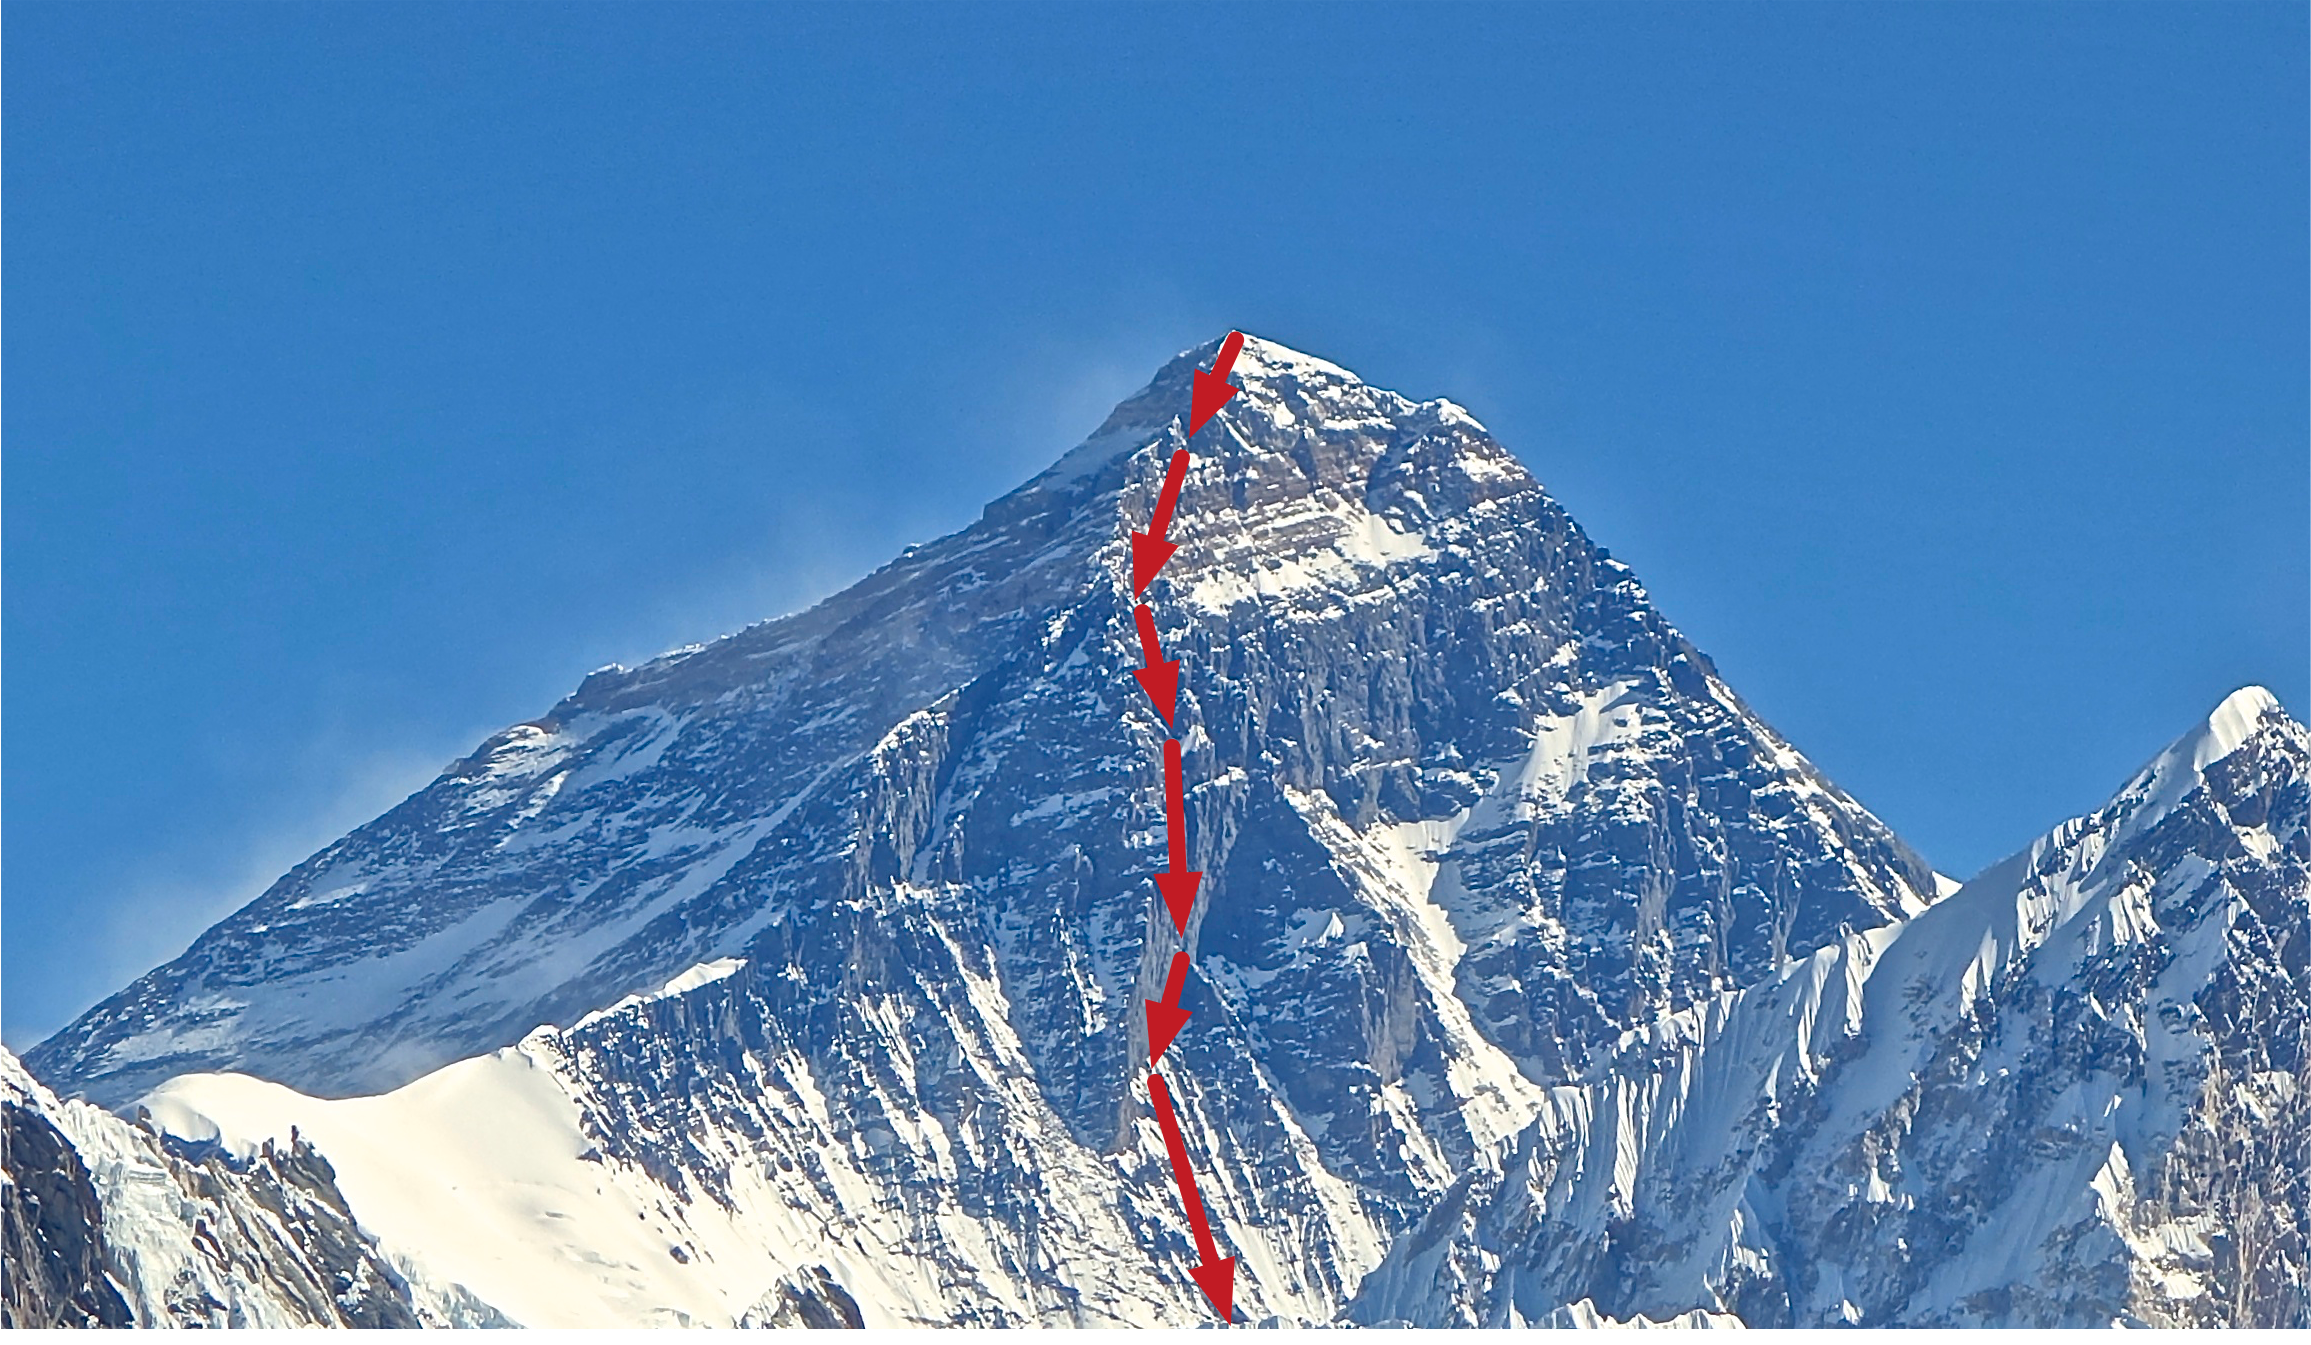
\includegraphics[width = 0.8\textwidth]{figure_man/linesearch.png}
			\hspace{2cm} \begin{footnotesize} "Walking down the hill, towards the valley." \end{footnotesize}\\
			\end{center}
		\end{column}
	\end{columns}
	
\framebreak

\begin{center}
$ $ \\
\includegraphics[width=0.8\textwidth]{figure_man/negative_gradients.png}
\end{center}

\end{vbframe}

\begin{vbframe}{Line search for smooth functions}

	In the following, let $f: \R^d \to \R$ be continuously differentiable.
	
	\lz
	
	\textbf{Definition:} A vector $\mathbf{d}\in \R^d /\ \{\mathbf{0}\}$ is called \textbf{descent direction} in $\xv$ if
	$$
	\nabla_{\mathbf{d}} f(\xv) = \nabla f(\xv) ^T \mathbf{d} < 0,
	$$
	
	i.e., the directional derivative at $\xv$ towards $\mathbf{d}$ is negative.
	(for the terminology, refer to chapter 1 \textbf{Mathematical concepts}.)
	\vspace*{-0.2cm}
	\begin{center}
		\includegraphics[width = 0.5\textwidth]{figure_man/descent_direction.png}
	\end{center}
	
	\framebreak
	
	Line search algorithms can be summarized as follows:
	\vspace*{-0.2cm}
	\begin{algorithm}[H]
	  \caption{Line search}
	  \begin{algorithmic}[1]
	  \State Choose a starting point $\xv^{[0]} \in \R^d$
	  \For {$t = 0, 1, 2, ...$}
	    \State Calculate a descent direction $\mathbf{d}^{[t]}$ for the current $\xv^{[t]}$:
	$$
	\nabla_{\mathbf{d}^{[t]}} f(\xv^{[t]}) = (\mathbf{d}^{[t]})^\top\nabla f(\xv^{[t]}) < \mathbf{0}
	$$
	    \State Find a $\alpha^{[t]}$ such that with $\xv^{[t + 1]} = \xv^{[t]} + \alpha^{[t]} \mathbf{d}^{[t]}$
	  the function value becomes smaller, i.e. $f(\xv^{[t + 1]}) < f(\xv^{[t]})$.
	    \State If no convergence has been achieved and the maximum number of iterations
	has not been exceeded, continue with step 2.
	  \EndFor
	  \end{algorithmic}
	\end{algorithm}
	\vspace*{-0.2cm}
	\begin{tiny}
		Please note that the terminology is misleading as ``line search'' on the one hand refers to Step 4 (selecting the step size that decreases $f(\xv)$) and on the other hand ``line search'' is the umbrella term for iterative algorithms that are based on finding a local minimum using descent methods. \par
	\end{tiny}
\end{vbframe}



\begin{vbframe}{Gradient Descent}

	Line search with the direction of the steepest descent (the negative gradient) is commonly referred to as \textbf{gradient descent} (GD). 

	\begin{center}
		$f(x_1, x_2) = - \sin(x_1) \cdot \frac{1}{2\pi} \exp\left( (x_2 - \pi / 2)^2 \right)$

		\begin{center}
			\includegraphics[width = 0.9\textwidth]{figure_man/example-descent1.png}
		\end{center}
		
	\end{center}

\end{vbframe}




\begin{vbframe}{Optimizing the linear model with GD}

	Given are $n$ observations $\D = \Dset$. We assume that the unknown connection between $\xv \in \R^p$ and $y\in \R$ can be described as $f(\xv) = y.$
	
	\vspace*{0.2cm}

	\textbf{Aim:} Find a good estimate for $f$ give $\D$. 

	\vspace*{0.2cm}

	\textbf{Approach:} We restrict $f$ to the hypothesis space of linear functions $\Hspace = \fxt = \{\thetab^{\top}\xv, \thetab \in \R^p\}$. We use the quadratic loss as a loss function, and minimize the resulting empirical risk
	
	\begin{eqnarray*}
	\argmin_{\thetab}\riske(\thetab) &=& \argmin_{\thetab} \sum_{i=1}^n \left(y^{(i)} - \fxit\right)^2 \\ &=& \argmin_{\thetab} \sum_{i=1}^n \left(y^{(i)} - \thetab^{\top} \xv^{(i)}\right)^2 \\
	\end{eqnarray*}
	
	% \begin{footnotesize}
	% $^{(*)}$To keep the notation simple, the intercept term is not explicitly written here. For an intercept term we simply define $\thetab \in \R^{p + 1}$ and define our data points $\tilde x^{(i)} = (1, x^{(i)}_1, ..., x^{(i)}_p)$.
	% \end{footnotesize}

	\framebreak
	
	The gradient of $\riskt$ is 	
	$$
	\nabla_{\thetab}\riske(\thetab) =  \frac{\partial \riske(\thetab)}{\partial
	\thetab} = - \sum_{i=1}^n 2 \cdot \left(y^{(i)} - \thetab^{\top} \xv^{(i)}\right) \xv^{(i)}.
	$$
	
	Therefore, an iteration of gradient descent is
	
	$$
	\thetatn \leftarrow \thetat + \alpha^{[t]} \sum_{i=1}^n 2 \cdot \left(y^{(i)} - \thetab^{[t]\top} \xv^{(i)}\right) \xv^{(i)}.
	$$
	
	$\alpha$ determines the length of the step and is called \textbf{step size} or, in risk minimization, \textbf{learning rate}.

	\lz 

	\begin{footnotesize}
	\textbf{Note: } For illustration, we optimize the linear model with quadratic loss with gradient descent, even though a closed-form solutions exists in this case. 
	\end{footnotesize}

	\framebreak
	
	
	\begin{center}
	$ $ \\
	\includegraphics[width=\textwidth]{figure_man/iter0.png}\\
	\begin{footnotesize}
	\end{footnotesize}
	\end{center}


	
	\framebreak
	
	\begin{center}
	$ $ \\
	\includegraphics[width=\textwidth]{figure_man/iter1.png}\\
	\begin{footnotesize}
	\end{footnotesize}
	\end{center}
	
	\framebreak
	
	\begin{center}
	$ $ \\
	\includegraphics[width=\textwidth]{figure_man/iter2.png}\\
	\begin{footnotesize}
	\end{footnotesize}
	\end{center}

\end{vbframe}

\endlecture
\end{document}

